\section{倾斜叠加}
\label{sec:5.2}

倾斜叠加是炮检距坐标轴的一种变换,它就像是对地震波束进行定向导引。我认为,过去
我引入术语倾斜叠加(slant stack)
只不过是把它作为以下\ref{sec:5.3}节中将述及之某种偏移方法的
一部分(Schultz与Claerbout,
1978),我确实未曾发明过倾斜叠加概念!上溯到Rieber教
授在1930年代的工作和苏联的Pa6nHKHH H.
A教授的工作,它在勘探地震学中已有一个很
长的历史了。从数学上说,倾斜叠加的概念在Radon变换(Radon,
1917)中就已奠定了基础。

倾斜叠加思想很类似于把出射角附近之数据加以组合的Snell记录道方法。Snell记录道
的思想是根据假想速度所预测出的局部时差$p=dt/dx$来选择数据,倾斜叠加却不是预测该
时差,而是进行滤波将该时差提取出来。因而,倾斜叠加不论速度是否已知均能正确地起作
用。在介质的速度是已知的时候,能够使倾斜叠加直接实现向下延拓,即使在有绕射和多次
反射的情形下出现混杂的视速度时,也能够如此。

\subsection{倾斜叠加与线性时差校正}
\label{sec:5.2.1}

在剖面或道集上寻找某种特定时差$p=dt/dx$的同相轴,相当于是对各双曲线同相轴进行
扫描以找出它们与斜率为夕之某条直线相切的地方,如利用线性时差校正将数据重新加以显
示,亦即,如将$(x,t)$平面内位于炮检距$x=g-s$和时间t上的能量转移至$(x,t')$
平面内位于炮检距x和时间$t'=t-px$
上,那末进行搜索和分析就会容易一些。这种转移过程如图
\ref{fig:slnt/lmo}所示,线性时差校正将$(x,t)$
平面内所有斜率为p的同相轴转换为$(x,t')$平面内
的“水平”同相轴,图中出现的水平计时线是为了方便于搜索和追踪测定同相轴位置。

\begin{figure}[H]
\centering
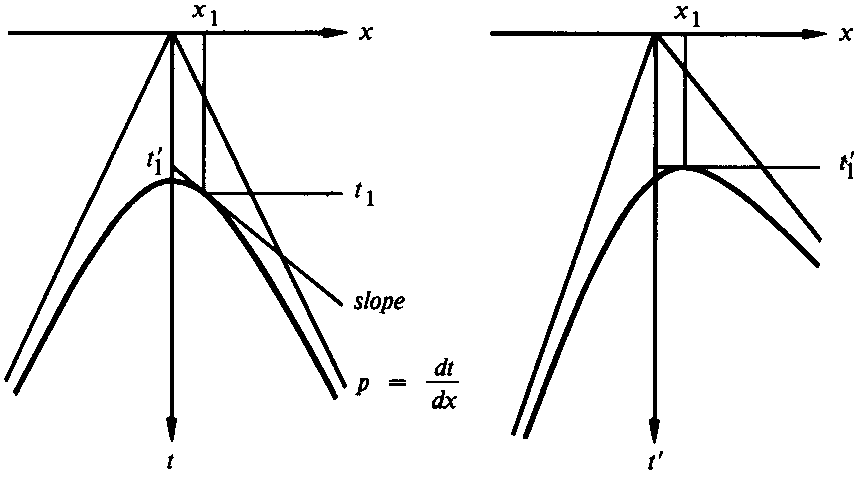
\includegraphics[width=0.65\textwidth]{slnt/lmo}
\caption[lmo]{线性时差校正将追踪识别与所构制平行直线相切之任务转
变成了给凸同相轴之顶部定位的任务}
\label{fig:slnt/lmo}
\end{figure}

在线性时差校正之后$t'=t-px$,具有Snell参量大约为p之数据中的各种组成成分就都
是沿x坐标作缓慢变化了。要提取它们,应对x坐标采用某种低通滤波处理,并对每一$t'$时间
值都如此作。低频滤波的极限情形就是提取均值,这就导致倾斜叠加的思想。

为进行倾斜叠加,要根据$t'=t-px$作线性时差校正,然后遍及x坐标求和,这样作的效
果与沿$(x,t)$平面内之倾斜直线进行求和是相同的。无论在哪种情形下,都能使整个道集
$P(x,t)$转换成作为时间广之函数的一个记录道。倾斜叠加假设遍及观测炮检距的求和可
适当代表沿炮检距坐标%的积分作用,沿炮检距坐标的倾斜积分所受到的主要影响将来自积
分路径与双曲面波至成为相切之处的区域;另一方面,在时距曲线与积分曲线相交时,对该
积分的影响就小到几乎等于零,原因就是传播之波没有零频率的成分。

波至的强度有赖于相切区域的长度,相切区长度的Fresnel定义是以半波长条件为基础
的。在速度为恒定值但有许多是平缓层的地层内,相切区之宽度因双曲线变平坦从而将随时
间而变宽,这种増宽与$\sqrt{t}$成比例,抵得上完成了一半的球面扩散校正。换言之,倾斜叠加
把我们从二维带到了一维世界,但是将三维的圆锥波阵面校正为二维的平面波还得再有个
$\sqrt{t}$。

\subsection{倾斜叠加道集是椭圆}
\label{sec:5.2.2}

数据道集的倾斜叠加产生一个以倾斜参量p为其特征的记录道,按许多p值进行倾斜叠加
处理则产生倾斜叠加道集。(具有坚实数学物理基础的读者们将会注意到,进行倾斜叠加其
实就是用Legendre变换将时距曲线加以变换,在这方面,特别条理清晰的背景读物是
H.B.Callen所著《热力学》[1960年Wiley公司出版,90页至95页])。
